\apendice{Especificación de Requisitos}

\section{Introducción}
En este anexo se va a realizar y formalizar la especificación de requisitos que define el comportamiento del sistema de desarrollo 
mediante el uso de tablas y diagramas.
\section{Objetivos generales}
Los objetivos que se persiguen en este proyecto son:
\begin{itemize}
	\item Desarrollar una herramienta que permita la extracción, el tratamiento y la subida de los datos de las plataformas correspondientes.
	\item Confeccionar esta herramienta de la manera más simple y transparente para el usuario.
	\item Almacenar todos los datos generados para futuros usos por parte del usuario.
\end{itemize}
\section{Catalogo de requisitos}
Se van a enumerar los requisitos específicos derivados de los objetivos del proyecto y que definen algún tipo de función dentro del mismo.
\subsection{Requisitos funcionales}
\begin{itemize}
	\item \textbf{RF-1} Introducir datos de búsqueda: el usuario debe de ser capaz de introducir los datos referentes al autor a buscar en las diferentes plataformas. 
	\item \textbf{RF-2} Cambiar datos de búsqueda: el usuario debe de ser capaz de volver a introducir los datos si el sistema detecta que ha habido algún problema con los datos previamente introducidos
	\item \textbf{RF-3} Subida de datos extraídos. El usuario debe de ser capaz de subir los datos a ACADEMIA, para ello debe identificarse en la aplicación web ACADEMIA.
	\begin{itemize}
		\item \textbf{RF-3.1} Datos erróneos: en caso de que los datos introducidos sean erróneos, impedir al acceso y solicitar de nuevo las credenciales.
		\item \textbf{RF-3.2} Datos correctos: en caso de que los datos sean correctos. Comenzar la subida de los datos.
	\end{itemize}
	\item \textbf{RF-4} Datos bibliográficos erróneos. El usuario debe de ser capaz de obtener los datos bibliográficos que no hayan podido ser subidos por erróneos o incompletos.
\end{itemize}
\subsection{Requisitos no funcionales}
\begin{itemize}
	\item \textbf{RNF-1 Usabilidad:} La herramienta ha de ser intuitiva y con una interfaz amigable.
	\item  \textbf{RNF-2 Escalabilidad} La herramienta ha de estar preparada para la adicción de nuevas funcionalidades
\end{itemize}
\section{Especificación de requisitos}
En este apartado se va a mostrar mediante diagramas los casos de uso de los requisitos previamente definidos, para ello se va a utilizar la notación \emph{UML}\cite{uml}.

\begin{figure}[H]
	\centering
	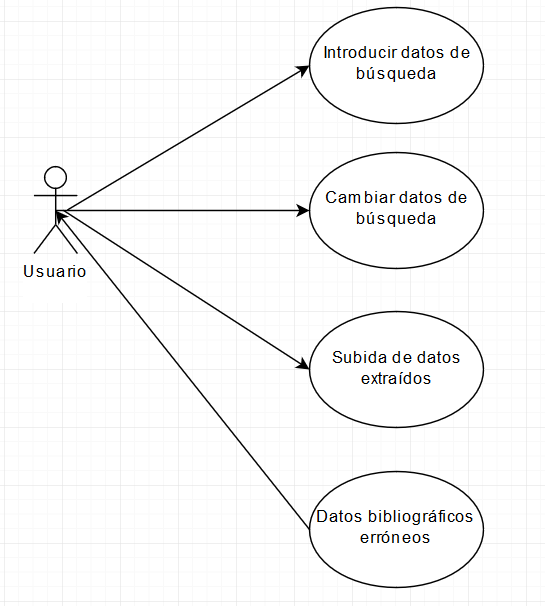
\includegraphics[width=0.8\textwidth]{UML1}
	\caption{Diagrama UML general de casos de uso.}
\end{figure}

\begin{figure}[H]
	\centering
	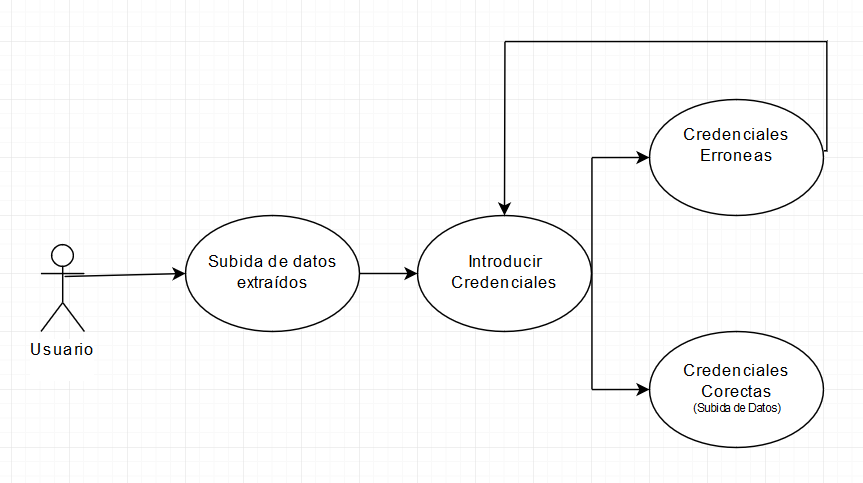
\includegraphics[width=1\textwidth]{UML2}
	\caption{Diagrama UML desglosado del caso de uso 3.}
\end{figure}

\tablaSmallSinColores{Caso de uso 1: Introducir datos de búsqueda}{p{3cm} p{.75cm} p{9.5cm}}{b1}{
	\multicolumn{3}{l}{Caso de uso 1: introducir datos de búsqueda} \\
}
{
	Descripción                            & \multicolumn{2}{p{10.25cm}}{El usuario debe introducir los datos referentes al autor a buscar} \\\hline
	\multirow{2}{3.5cm}{Requisitos}  &\multicolumn{2}{p{10.25cm}}{RF-1} \\\cline{2-3}
	\\\hline
	Precondiciones                         &   Ninguna   & 
	\\\hline
	\multirow{2}{3.5cm}{Secuencia normal}  & Paso & Acción \\\cline{2-3}
	& 1    & El usuario inicia la herramienta. 
	\\\cline{2-3}
	& 2    & El usuario introduce el nombre de autor para \emph{Google Scholar}.
	\\\cline{2-3}
	& 3    & El usuario introduce el \emph{author ID} para \emph{Scopus}.
	\\\cline{2-3}
	& 4    & El usuario introduce el nombre de autor para \emph{Web of Science}.
	\\\cline{2-3}
	& 5    & El usuario pulsa el botón \emph{Search} para comenzar la búsqueda.                                  	 
	\\\hline
	Postcondiciones                        & \multicolumn{2}{p{10.25cm}}{Se produce un cambio en la interfaz que indica al usuario que el proceso de búsqueda a comenzado} \\\hline
	Excepciones                        & \multicolumn{2}{p{10.25cm}}{Ninguna}\\\hline
	Importancia                            & Alta \\\hline
	Urgencia                               & Alta \\\hline
	Comentarios                            & & \\
}

\tablaSmallSinColores{Caso de uso 2: cambiar datos de búsqueda}{p{3cm} p{.75cm} p{9.5cm}}{b1}{
	\multicolumn{3}{l}{Caso de uso 2: Cambiar datos de búsqueda} \\
}
{
	Descripción                            & \multicolumn{2}{p{10.25cm}}{El usuario debe introducir los datos que se han introducido de forma errónea o que no han producido resultados} \\\hline
	\multirow{2}{3.5cm}{Requisitos}  &\multicolumn{2}{p{10.25cm}}{RF-1,RF-2} \\\cline{2-3}
	\\\hline
	Precondiciones                         & \multicolumn{2}{p{10.25cm}}{Se ha llevado a cabo RF-1} 
	\\\hline
	\multirow{2}{3.5cm}{Secuencia normal}  & Paso & Acción \\\cline{2-3}
	& 1    & Se detecta un error con los datos introducidos. 
	\\\cline{2-3}
	& 2    & Se muestra una nueva entrada de datos, correspondiente al proceso que se está llevando a cabo.
	\\\cline{2-3}
	& 3    & El usuario introduce los datos.
	\\\cline{2-3}
	& 4    & El proceso de búsqueda es reactivado con los nuevos datos.                                 	 
	\\\hline
	Postcondiciones                        & \multicolumn{2}{p{10.25cm}}{Se reanuda el proceso de búsqueda y se produce un cambio en la interfaz que indica al usuario que este ha sido reactivado} \\\hline
	Excepciones                        & \multicolumn{2}{p{10.25cm}}{Ninguna}\\\hline
	Importancia                            & Alta \\\hline
	Urgencia                               & Alta \\\hline
	Comentarios                            & & \\
}

\tablaSmallSinColores{Caso de uso 3: subida de datos extraídos}{p{3cm} p{.75cm} p{9.5cm}}{b1}{
	\multicolumn{3}{l}{Caso de uso 3: Subida de datos extraídos} \\
}
{
	Descripción                            & \multicolumn{2}{p{10.25cm}}{El usuario debe introducir las credenciales de acceso a ANECA, para iniciar el proceso de subida de los datos previamente extraídos } \\\hline
	\multirow{2}{3.5cm}{Requisitos}  &\multicolumn{2}{p{10.25cm}}{RF-3} \\\cline{2-3}
	\\\hline
	Precondiciones                         & \multicolumn{2}{p{10.25cm}}{Se ha llevado a cabo RF-1} 
	\\\hline
	\multirow{2}{3.5cm}{Secuencia normal}  & Paso & Acción \\\cline{2-3}
	& 1    & Se introduce las credenciales de acceso. 
	\\\cline{2-3}
	& 2    & Se comprueba que las credenciales son correctas.
	\\\cline{2-3}
	& 3    & Se activa el proceso de subida de los datos a la aplicación virtual.                               	 
	\\\hline
	Postcondiciones                        & \multicolumn{2}{p{10.25cm}}{Se  produce un cambio en la interfaz que indica al usuario que el proceso se está llevando a cabo} \\\hline
	Excepciones                        & \multicolumn{2}{p{10.25cm}}{Ninguna}\\\hline
	Importancia                            & Alta \\\hline
	Urgencia                               & Alta \\\hline
	Comentarios                            & & \\
}
\tablaSmallSinColores{Caso de uso 3.1: Credenciales erróneas }{p{3cm} p{.75cm} p{9.5cm}}{b1}{
	\multicolumn{3}{l}{Caso de uso 3.1: credenciales erróneas} \\
}
{
	Descripción                            & \multicolumn{2}{p{10.25cm}}{La herramienta debe identificar que las credenciales introducidas son erróneas y ofrecer la posibilidad de volver a introducirlas.} \\\hline
	\multirow{2}{3.5cm}{Requisitos}  &\multicolumn{2}{p{10.25cm}}{RF-3.1} \\\cline{2-3}
	\\\hline
	Precondiciones                         & \multicolumn{2}{p{10.25cm}}{Se ha llevado a cabo RF-3} 
	\\\hline
	\multirow{2}{3.5cm}{Secuencia normal}  & Paso & Acción \\\cline{2-3}
	& 1    & Se comprueba que las credenciales son erróneas \emph{.bib}. 
	\\\cline{2-3}
	& 2    & Se ofrece la posibilidad al usuario de volver a introducirlas.                              	 
	\\\hline
	Postcondiciones                        & \multicolumn{2}{p{10.25cm}}{Ninguna} \\\hline
	Excepciones                        & \multicolumn{2}{p{10.25cm}}{Ninguna}\\\hline
	Importancia                            & Alta \\\hline
	Urgencia                               & Alta \\\hline
	Comentarios                            & & \\
}

\tablaSmallSinColores{Caso de uso 3.2: Credenciales correctas }{p{3cm} p{.75cm} p{9.5cm}}{b1}{
	\multicolumn{3}{l}{Caso de uso 3.2: credenciales correctas} \\
}
{
	Descripción                            & \multicolumn{2}{p{10.25cm}}{La herramienta debe identificar que las credenciales introducidas son correctas y comenzar el proceso de subida de datos.} \\\hline
	\multirow{2}{3.5cm}{Requisitos}  &\multicolumn{2}{p{10.25cm}}{RF-3.2} \\\cline{2-3}
	\\\hline
	Precondiciones                         & \multicolumn{2}{p{10.25cm}}{Se ha llevado a cabo RF-3} 
	\\\hline
	\multirow{2}{3.5cm}{Secuencia normal}  & Paso & Acción \\\cline{2-3}
	& 1    & Se comprueba que las credenciales son correctas \emph{.bib}. 
	\\\cline{2-3}
	& 2    & Se comienza el proceso de subida de datos.                              	 
	\\\hline
	Postcondiciones                        & \multicolumn{2}{p{10.25cm}}{Cambio en la interfaz que indica al usuario que el proceso de subida se está llevando a cabo} \\\hline
	Excepciones                        & \multicolumn{2}{p{10.25cm}}{Ninguna}\\\hline
	Importancia                            & Alta \\\hline
	Urgencia                               & Alta \\\hline
	Comentarios                            & & \\
}

\tablaSmallSinColores{Caso de uso 4: Datos bibliográficos erróneos}{p{3cm} p{.75cm} p{9.5cm}}{b1}{
	\multicolumn{3}{l}{Caso de uso 4: datos bibliográficos erróneos} \\
}
{
	Descripción                            & \multicolumn{2}{p{10.25cm}}{La herramienta debe guardar e informar al usuario de los datos bibliográficos que no han podido ser subidos a ACADEMIA } \\\hline
	\multirow{2}{3.5cm}{Requisitos}  &\multicolumn{2}{p{10.25cm}}{RF-3} \\\cline{2-3}
	\\\hline
	Precondiciones                         & \multicolumn{2}{p{10.25cm}}{Se ha llevado a cabo RF-3} 
	\\\hline
	\multirow{2}{3.5cm}{Secuencia normal}  & Paso & Acción \\\cline{2-3}
	& 1    & Se almacenan los datos erróneos en un fichero \emph{.bib}. 
	\\\cline{2-3}
	& 2    & Se notifica al usuario del número de datos que no han podido ser subidos.                              	 
	\\\hline
	Postcondiciones                        & \multicolumn{2}{p{10.25cm}}{Ninguna} \\\hline
	Excepciones                        & \multicolumn{2}{p{10.25cm}}{Ninguna}\\\hline
	Importancia                            & Alta \\\hline
	Urgencia                               & Alta \\\hline
	Comentarios                            & & \\
}
